\subsection{Model Validation}
\label{subsec:model_validation}

Achieving a good in-sample fit does not necessarily guarantee that our model will also be
able to make out of sample predictions. For example, it could be that the results are
very sensitive to the exact number of vaccinations, the work mobility multiplier
($\rho_{w,\:attend,\:t}$) or the number of rapid tests (governed by the $\pi$ parameters)
that are performed -- all of which are things that cannot be known exactly ex-ante.

In this section we compare simulated infections that use all available data with
out of sample predictions that only use data that was available at March 1 2021.

For the out of sample predictions we predict the number of vaccinations between March and
June with a simple linear regression model that was fitted on vaccine data from February.
This prediction model is pessimistic compared to the actual number of vaccinations. The
work mobility multiplier ($\rho_{w,\:attend,\:t}$) is predicted to be constant at a value
of 0.75, which is an approximate average of the second half of February. This turned out
to be optimistic.

The area that is fraught with the most uncertainty is the introduction of rapid tests,
because it comprises both supply and demand factors. Moreover, accurately predicting the
number of rapid tests is expected to be important because rapid tests play a large role
for the transmission dynamic.

We therefore make a scenario analysis with different assumptions on the availability of
rapid tests. The number of rapid tests performed in each scenario can be seen in
Figure~\ref{fig:robustness_check_rapid_test_params}. All scenarios are the same until
March 1 and have the same level of rapid tests when all supply constraints are resolved.
They differ in the date at which the full number of tests is reached. For students
($\pi_{students,\:t}$) and teachers ($\pi_{teacher,\:t}$) the full number of rapid tests
is reached after the Easter holidays in all scenarios. For rapid tests in the workplace
($\pi_{w,\:s,\:t}$) and private rapid tests ($\pi_{private,\:t}$) it is reached between
May 1 and June 10, depending on the scenario.


\begin{figure}[ht] % Robustness Check Rapid Test Fade In Params
  \centering
  \begin{subfigure}[b]{0.3\textwidth}
    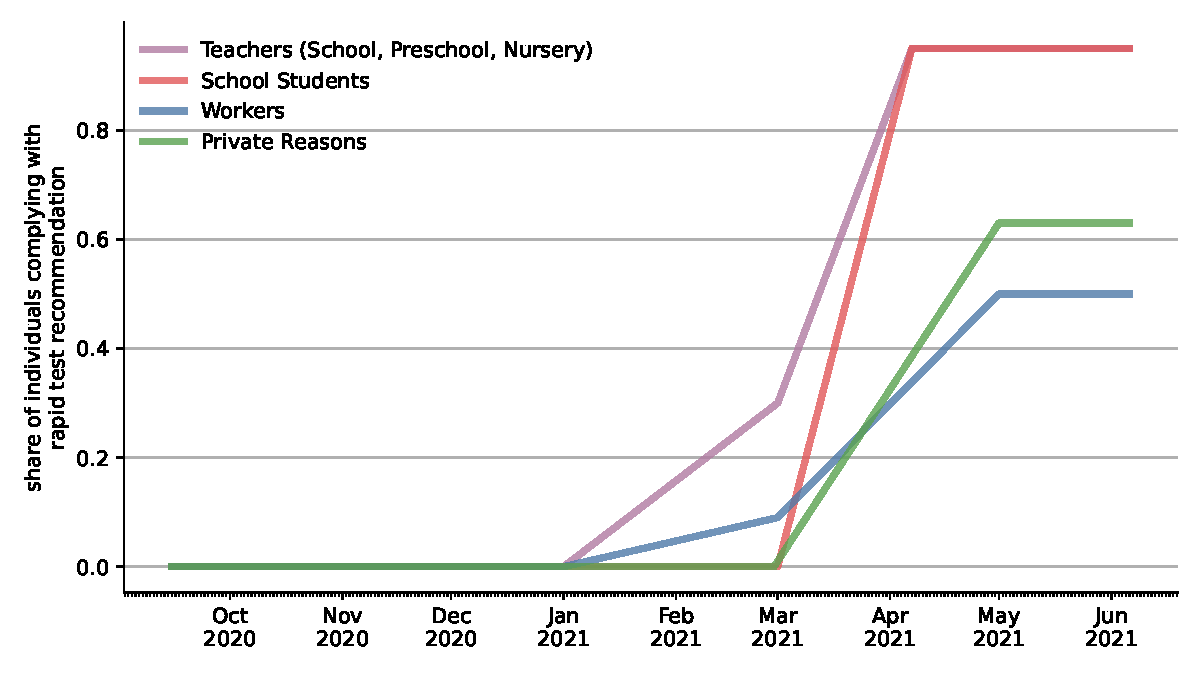
\includegraphics[width=\textwidth]{figures/results/figures/data/testing/rapid_test_demand/robustness_check_params_early_shares}
    \caption{Rapid Test Parameters: Early Scenario}
    \label{fig:robustness_early_params}
  \end{subfigure}
  \hfill
  \begin{subfigure}[b]{0.3\textwidth}
    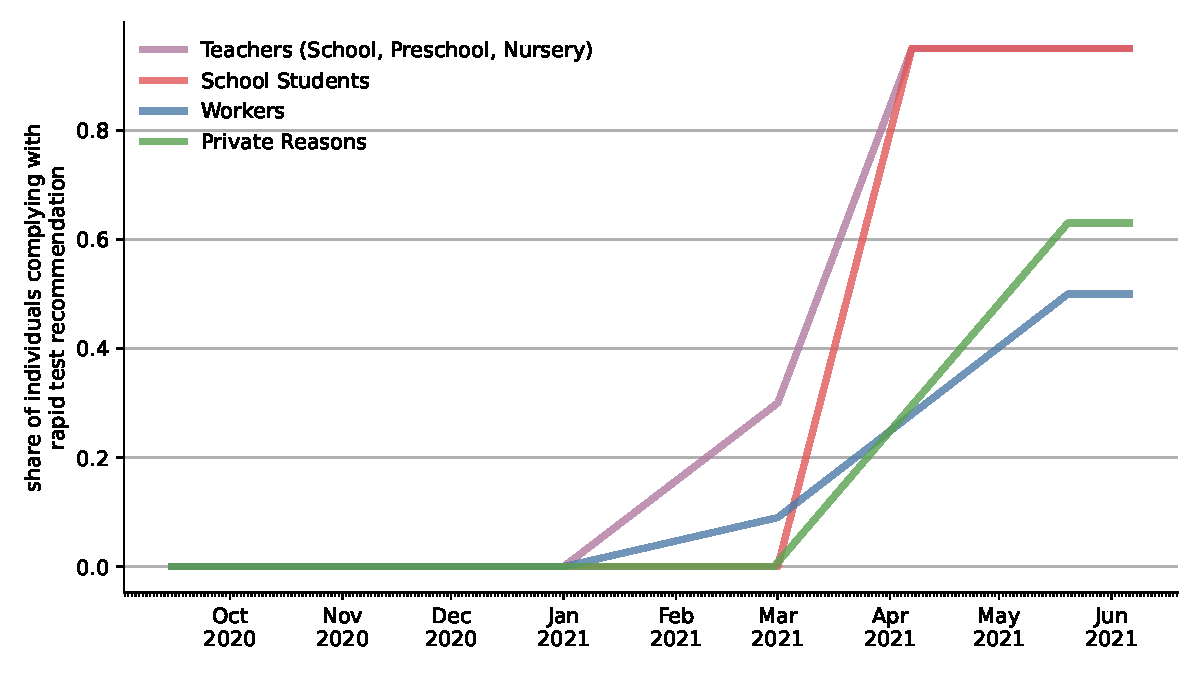
\includegraphics[width=\textwidth]{figures/results/figures/data/testing/rapid_test_demand/robustness_check_params_medium_shares}
    \caption{Rapid Test Parameters: Medium Scenario}
    \label{fig:robustness_medium_params}
  \end{subfigure}
  \hfill
  \begin{subfigure}[b]{0.3\textwidth}
    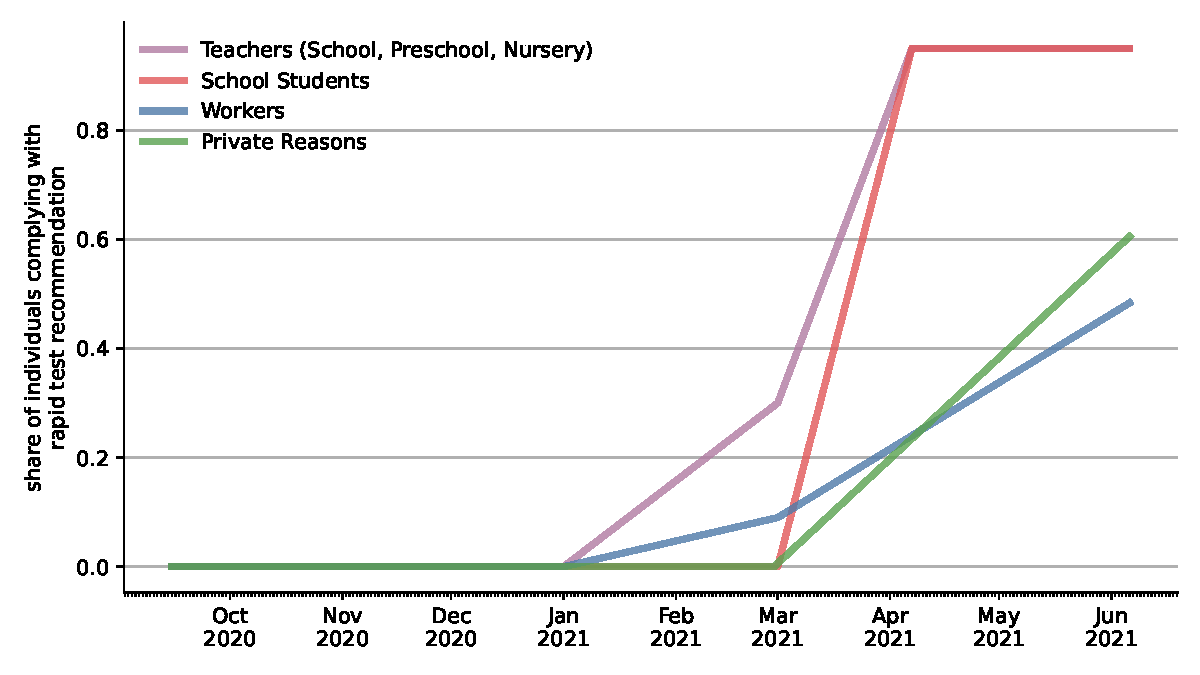
\includegraphics[width=\textwidth]{figures/results/figures/data/testing/rapid_test_demand/robustness_check_params_late_shares}
    \caption{Rapid Test Parameters: Late Scenario}
    \label{fig:robustness_late_params}
  \end{subfigure}

  \caption{Rapid Test Introduction in the Three Scenarios}
  \label{fig:robustness_check_rapid_test_params}

  \floatfoot{\noindent \textit{Note:} Number of rapid tests performed in the different
  prediction scenarios. All scenarios are the same until March 1 and have the same level
  of rapid tests when all supply constraints are resolved. They differ in the date at
  which the full number of tests is reached. For students ($\pi_{students,\:t}$) and
  teachers ($\pi_{teacher,\:t}$) the full number of rapid tests is reached after the
  Easter holidays in all scenarios. For rapid tests in the workplace ($\pi_{w,\:s,\:t}$)
  and private rapid tests ($\pi_{private,\:t}$) it is reached between May 1 and June 10,
  depending on the scenario.}
\end{figure}

Moreover, the out of sample predictions assume that the share of detected cases
($\psi_t$) that would have been obtained without rapid tests is not affected by the
Easter holidays because the extent to which this was the case was estimated from case
numbers in April.

The results of the out of sample prediction are displayed in
Figure~\ref{fig:robustness_check_detailed}. While all scenarios considerably deviate from
the ex-post scenario, they all reproduce the steep increase of cases until the end of
April, followed by a decline until June. We can therefore conclude that our main results
are not sensitive to measurement errors in the number of rapid tests, vaccinations or
mobility data.


\begin{figure}[ht] % Robustness Check
  \centering
  \begin{subfigure}[b]{.425\textwidth}
    \centering
    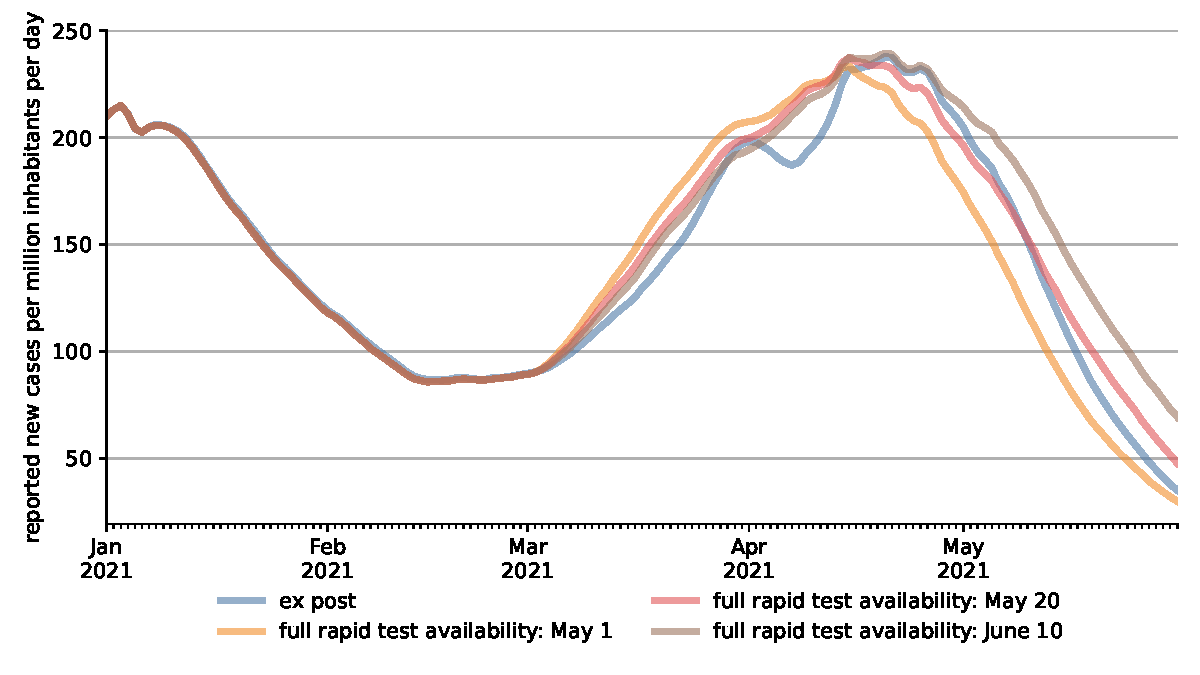
\includegraphics[width=\textwidth]{figures/results/figures/scenario_comparisons/robustness_check/full_new_known_case}
    \caption{Reported Cases}
    \label{fig:robustness_check_new_known_case}
  \end{subfigure}%
  \hfill
  \begin{subfigure}[b]{.425\textwidth}
    \centering
    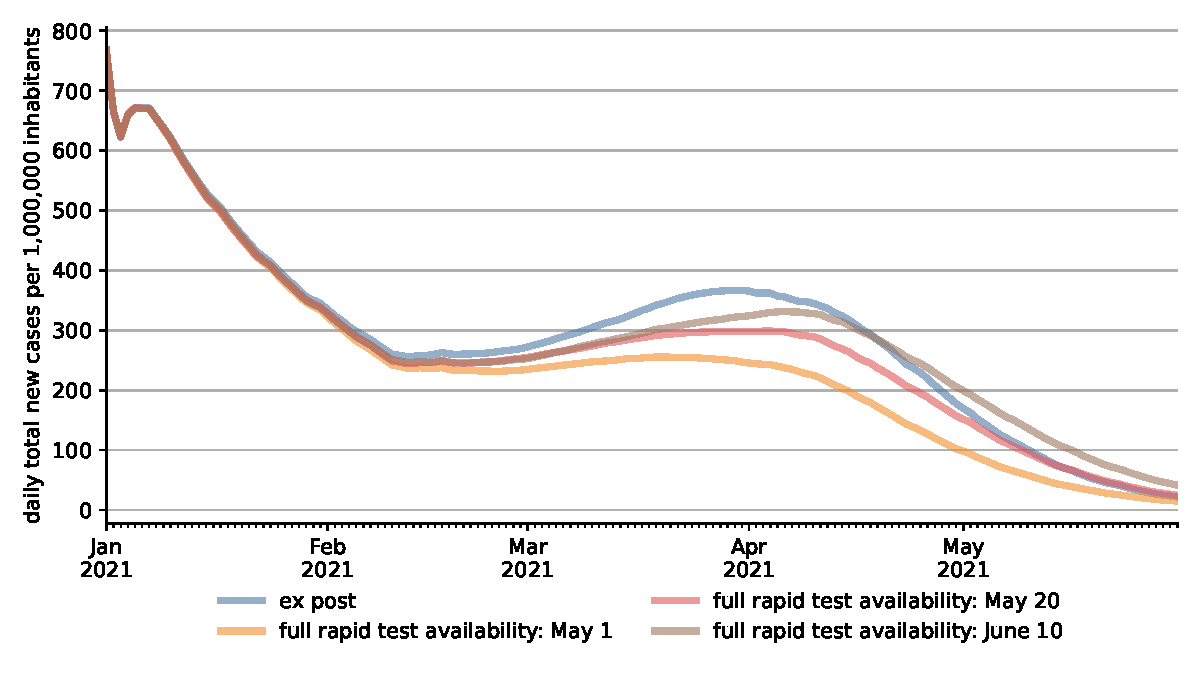
\includegraphics[width=\textwidth]{figures/results/figures/scenario_comparisons/robustness_check/full_newly_infected}
    \caption{Total Cases}
    \label{fig:robustness_check_newly_infected}
  \end{subfigure}
  \caption{Out of Sample Prediction for Reported and Total Cases from March to June
  2021.}
  \label{fig:robustness_check_detailed}
  \floatfoot{\noindent \textit{Note:} The ex-post scenario is an in-sample prediction
  that uses all available information and is very close to actual case numbers. For the
  other scenarios data on vaccinations, work mobility and rapid tests that became
  available after March 1 have been replaced by prediction models that are calibrated
  with data from February. Moreover, they do not model a lower number of detected cases
  over the Easter holidays. The different scenarios make different assumptions on the
  date at which full availability of rapid tests is reached. While the out of sample
  predictions differ substantially for the exact case numbers at the beginning of June
  (between 20 and 70 cases per million), they can all reproduce the decline in case
  numbers that is jointly driven by seasonality, large scale rapid tests and
  vaccinations. For legibility reasons, all lines are rolling 7-day averages.}
\end{figure}

Another form of validating our model is to see how well our main results align with
other studies that evaluate the effect of large scale rapid testing. Of course, this
has to be taken with a grain of salt as the effect of any rapid testing policy depends
on the incidence of the disease in the population, how well other testing policies
such as PCR tests are working, the effect of seasonality and NPIs that are in place.

Nevertheless, it is reassuring that other studies find effect sizes in the same order
of magnitude.

\citet{Pavelka2021} estimates that a mass testing campaign in Slovakia in October and
November 2020 where approximately 65 \% of the population took a rapid test within a two
week period lead to a reduction in case numbers of 70 \% three weeks after the start
of the intervention. Moreover, they find that this strong reduction in
cases cannot be explained by isolation of people who tested positive alone but only when
they took into account that household members of people who tested positive reduced
their contacts.

While we do not model the exact scenario of \citet{Pavelka2021}, we can roughly compare
their estimates with our predictions for the difference between the baseline scenario
and and a scenario without rapid tests. In May about 45\% of people do
at least one rapid test in every week. Taking into account that there are many repeated
testers the number of people who do a test within a two week period is probably
slightly less than the 65 \% from the intervention in Slovakia. On the other hand, we
have many people who do more than one rapid test in that time which also leads to the
detection of cases. Our model predicts that the observed incidence with tests is
approximately 65 \% lower than without tests after three weeks.
Thus we have an effect size in the same order of magnitude but are slightly
less optimistic regarding the efficiency of rapid test.

\citet{Berger2021} analyse the effect of twice weekly rapid testing in schools. They
have two main findings: Firstly, rapid tests reduced the share of undetected cases
among students by a factor between 2 and 4. Secondly, open schools with mandatory
testing might leads to the same or even lower numbers of infections than closed
schools. The estimates are based on infection numbers after the Easter holiday.

Again, we do not directly simulated their scenarios but can roughly compare our results
to theirs. We estimate a share of undetected cases of approximately 75 \% among school
age children (5 to 14 years) at the beginning of April, see
Figure~\ref{fig:share_known_cases_by_age_group}. This drops to slightly less than 40 \%
at the end of our simulation period. Thus in the long run, mandatory tests at schools
led to a reduction of the share of undetected cases by a factor of more than 1.8 which
is just slightly below the factor of 2 to 4 predicted by \citet{Berger2021}.

Similarly we are slightly less optimistic for the effect opening schools with testing
compared to closing schools. While they predict that opening schools could even be
beneficial we estimate that it would lead to a slight increase in case numbers
see Figure~\ref{fig:school_scenarios_detailed}).



% In May 45 % per week are tested
% Incidence pessimistic = 1750
% Incidence with mass testing = 750


\FloatBarrier
